\section{BERT} \label{sec:BERT}

\subsection{Problem with ELMo} \label{sec:ProblemWithELMo}

Simple word embedding models, unlike \hyperref[sec:LSTM]{LSTM}s, cannot capture combinations of words, negation and \hyperref[sec:Polysemy]{polysemy}. But \hyperref[sec:LanguageModels]{language models} have been effective at \emph{sentence-level} nlp tasks like natural language inference and paraphrasing, which predict sentence relationships, and also \emph{token-level} tasks like \nameref{nlptask:namedentityrecognitionNER} and \nameref{nlptask:questionansweringQA}, where a fine-grained approach is needed (Devlin et al., 2019).   

Previous methods like \textbf{ULMFiT} and \nameref{sec:ELMo} use a \hyperref[sec:BidirectionalLM]{bidirectional language model (biLM)} to account for left and right context. But the problem is that neither the \hyperref[sec:ForwardLM]{forward} \hyperref[sec:LSTM]{LSTM} nor the \hyperref[sec:BackwardLM]{backward} \hyperref[sec:LSTM]{LSTM} account for past and future tokens \textbf{\textit{at the same time.}} This deficiency does not let the model perform as well as it should since information from the entire sentence is not being used \textbf{\textit{simultaneously}}, regardless of position. 


\begin{figure}[h]
\vspace{-5pt}
\centering
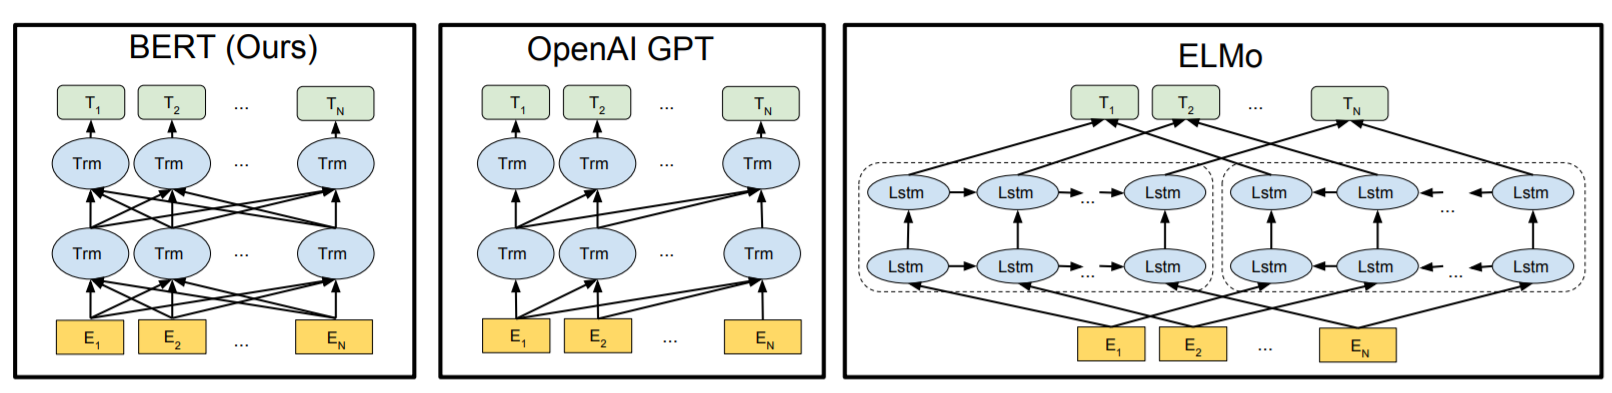
\includegraphics[width=0.9\textwidth]{imgs/bert_vs_elmo_vs_gpt.png}
\vspace{-5pt}
\caption{\footnotesize Comparing pre-training models: BERT uses a \hyperref[sec:BidirectionalLM]{bidirectional} \nameref{sec:Transformer}. OpenAI GPT uses a \hyperref[sec:ForwardLM]{forward} \nameref{sec:Transformer}. \nameref{sec:ELMo} combines independently-trained \hyperref[sec:ForwardLM]{forward} and \hyperref[sec:BackwardLM]{backward} \hyperref[sec:LSTM]{LSTM}s. Among the three, only BERT embeddings are jointly conditioned on forward and backward context in all layers. Alongside architectural differences, BERT and OpenAI GPT are fine-tuning approaches, while ELMo is a feature-based approach (Devlin et al., 2019). \textit{NOTE: $E_n =$ the $n$-th token in the input sequence, and $T_n =$ the corresponding output embedding}. From \emph{BERT: Pre-training of Deep Bidirectional Transformers for Language Understanding}, by Devlin et al., 2019. \url{https://arxiv.org/pdf/1810.04805.pdf}. Copyright 2019 by Devlin et al.}
\vspace{-5pt}
\label{fig:NAME}
\end{figure}





\subsection{Motivation for BERT} \label{sec:MotivationForBERT}

Instead of using \nameref{sec:ELMo}'s ``shallow" combination of ``independently-trained" \hyperref[sec:BidirectionalLM]{biLM}s, ``BERT is designed to pre-train deep bidirectional representations from unlabeled text by jointly conditioning on both left and right context in all layers" (Devlin et al., 2019).   


Another motivation for BERT stems from previous limitations. The \textbf{OpenAI GPT} model uses a left-to-right construction, where each token only attends to past tokens in the \hyperref[sec:SelfAttention]{self attention} layers of the \nameref{sec:Transformer}. This approach performs poorly on \emph{sentence-level} and \emph{token-level} tasks, like \nameref{nlptask:questionansweringQA}, where \textbf{bidirectional context} is required.  

\textbf{BERT (Bidirectional Encoder Representations from Transformers)} has progressed over past models since, in conjunction with its \hyperref[sec:BidirectionalLM]{biLM}, \hyperref[sec:SelfAttention]{self attention}, and \nameref{sec:Transformer} (more powerful than \hyperref[sec:LSTM]{LSTM}s), BERT uses a \hyperref[sec:maskedlanguagemodelMLM]{masked language model (MLM)} to avoid unidirectionality, resulting in vast performance gains over previous models (Wiedemann et al., 2019). 




\subsection{Describing BERT} \label{sec:DescribingBERT}

\subsubsection{Input Embedding in BERT} \label{sec:BERTInputEmbedding}

The input embedding in BERT is created by summing three kinds of other embeddings: 

\begin{enumerate}
    \item \textbf{\textit{WordPiece} token embeddings: }The \emph{WordPiece} \nameref{nlptask:tokenization} strategy, instead of tokenizing by the natural separations between English words, subdivides words into smaller, basic units. For example, the WordPiece \nameref{nlptask:tokenization} of ``playing" might be ``play" + ``**ing". This allows BERT to handle rare, unknown words (Weng, 2019) and reduce vocabulary size while increasing amount of data available per word. Consider: if ``play" and ``**ing" and ``**ed" are present in the vocabulary but ``playing" and ``played" are not, then these can be recognized by their sub-units. 
    
    \item \textbf{Segment embeddings: }are  arbitrary spans of contiguous text, rather than discrete sentences. The term ``sequence" for BERT refers to the input tokens, which can be parts of sentences or several sentences packed together. Contrary to BERT,  \nameref{sec:TransformerXL}'s \textbf{segment embeddings} respect sentence boundaries. 
    
    \item \textbf{\hyperref[sec:PosEncodings]{Positional embeddings}: } to account for word ordering. 
\end{enumerate}


\subsubsection{BERT's Framework}
 
There are two steps in BERT's framework: \textbf{pre-training}, in which BERT is trained on \emph{unlabeled data} over different tasks, and \textbf{fine-tuning}, in which BERT is initialized with the pre-training parameters to train over \emph{labeled data} for specific \hyperref[app:Appendix_NLPTasks]{nlp tasks}. Pre-training BERT using the \nameref{sec:maskedlanguagemodelMLM} task and \nameref{sec:nextsentencepredictionNSP} task allows BERT to learn \textbf{bidirectional context} and \emph{sentence-level} information, rather than just predict subsequent tokens given some context, as was the norm for simple \hyperref[sec:LanguageModels]{language models}.


\subsubsection{Masked Language Model (MLM)} \label{sec:maskedlanguagemodelMLM}

It is a well-known problem that bidirectional conditioning causes lower layers to leak information about tokens, so each word can implicitly ``see itself" letting the model trivially guess the target word in a multi-layered context (Devlin et al., 2019).  

BERT's solution is to use a \textbf{masked language model (MLM)}, which randomly masks some of the input tokens with the aim of predicting the original vocabulary id of the masked word using only its context. This fuses left and right context to get \emph{deep} bidirectional context, unlike \nameref{sec:ELMo}'s shallow left-to-right language model (Devlin et al., 2019).  

An issue with masking is that the model only predicts the \texttt{[MASK]} token when it is present in the input, while the intention was for the model to predict the correct tokens regardless of which tokens were present in input (Kurita, 2019a). This hampers performance since BERT would learn a contextual meaning of the mask token, causing it to learn slower since only $15 \%$ of tokens are masked. To resolve this, BERT varies its masking strategy: (1) replace the word to be masked with \texttt{[MASK]} only with $80\%$ probability; (2) replace the word to be masked with a random word $10 \%$ of the time; and (3) keep the masked word $10 \%$ of the time. For example, if the sentence was ``The cow jumped over the moon," and if the token to be masked was ``moon", then $80 \%$ of the time, the replacement would be ``The cow jumped over the \textbf{\texttt{[MASK]}}"; $10 \%$ of the time a random token would be used ``The cow jumped over the \textbf{seaweed}"; and the remaining times the sentence would remain the same. 



\subsubsection{Next Sentence Prediction (NSP)} \label{sec:nextsentencepredictionNSP}

Ordinary \hyperref[sec:LanguageModels]{language models} perform badly for tasks like \nameref{nlptask:questionansweringQA} and \nameref{nlptask:naturallanguageinferenceNLI} which require modeling sentence relationships, therefore BERT is pre-trained on a \textbf{next sentence prediction (NSP)} task for finding whether one sentence is the next sentence of the other. 

Training BERT using NSP is as follows: (1) sample sentence pairs \texttt{(A, B)} so that half the time \texttt{B} follows \texttt{A} (labeled as \texttt{IsNext}) and half the other time, \texttt{B} does not follow \texttt{A} (labeled as \texttt{NotNext}), then (2) BERT processes both sentences and uses a binary classifier to decide of \texttt{B} is the next sentence after \texttt{A} (Weng, 2019). 


\subsection{Experimental Results of BERT} \label{sec:BERTExperimentalResults}

% NOTE: the top width must be +0.5 more than below texwidth measure
\begin{program}
\begin{wrapfigure}{L}{0.75\textwidth}
    \begin{center}
    \vspace{-10pt}
    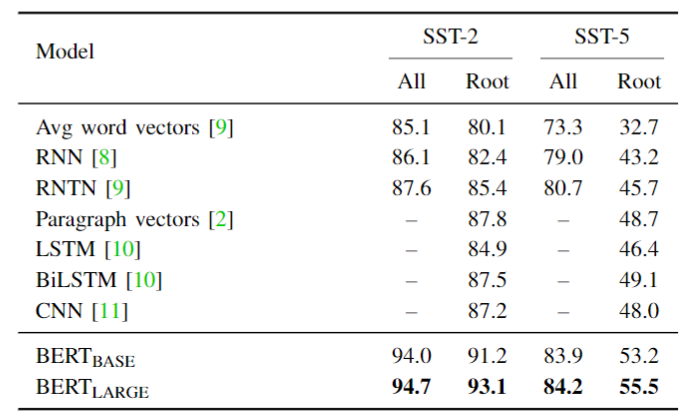
\includegraphics[width=0.6\textwidth]{imgs/table_bert_vsOtherModels.png}
    \end{center}
\vspace{-30pt}
\captionof{table}{\footnotesize Accuracy (\%) of several models on \nameref{nlptask:sentimentclassificationSC} SST dataset. BERT has highest accuracy scores. From \emph{Table B.II in Fine-Grained Sentiment Classification Using BERT}, by Munikar et al., 2019. \url{https://arxiv.org/pdf/1910.03474.pdf}. Copyright 2019 by Munikar et al.}
\label{tbl:bertExperimentResults}
\end{wrapfigure}


Using a simple accuracy measure, Munikar et al. (2019) found that a pre-trained BERT model fine-tuned for \nameref{nlptask:sentimentanalysisSA} task outperformed complex models such as \hyperref[sec:RNN]{RNN}s and CNNs. The \cref{tbl:bertExperimentResults} includes results on phrases and entire reviews. 


This proves \nameref{nlptask:transferlearning} is possible with BERT's deep contextual \hyperref[sec:BidirectionalLM]{bidirectional language model}.
\end{program}


\subsection{Probing BERT} \label{sec:ProbingBERT}

BERT has surpassed state-of-the-art performance in a wide range of \hyperref[app:Appendix_NLPTasks]{nlp tasks} but it is not known why. Clark et al. (2019) use an ``attention-based probing classifier" to study BERT's internal vector representations to understand what kinds of linguistic features BERT learns from its self-supervised training on unlabeled data. 



\subsubsection{BERT Learns Dependency Syntax} \label{sec:BERTLearnsSyntax}

Firstly, Clark et al. (2019) found that BERT's attention heads behave similarly, like focusing on positional offsets or attending broadly over an entire sentence. 

Secondly, while individual attention heads do not capture syntax dependency structure as a whole, it was found that certain attention heads are better at detecting various syntax dependency relations. For example, the heads detect ``direct objects of verbs, determiners of nouns, objects of prepositions, and objects of possessive pronouns with > $75 \%$ accuracy (Clark et al., 2019). 

\begin{figure}
\centering
\begin{minipage}{.4\textwidth}
  \centering
  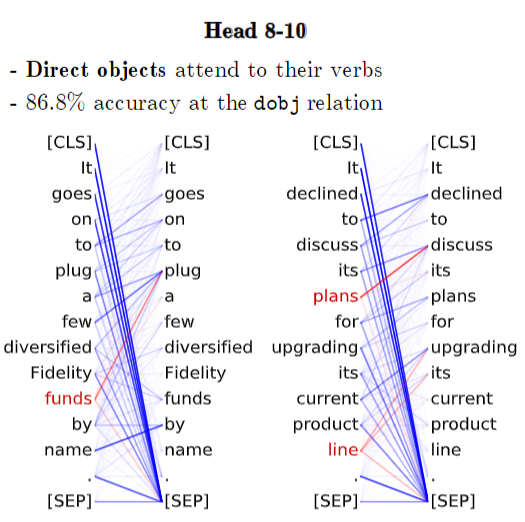
\includegraphics[width=\textwidth]{imgs/bert_headsDirectObject.png}
  \captionof{figure}{\footnotesize BERT attention heads capture syntax. In heads 8-10, direct objects are found to attend to their verbs. Line darkness indicates attention strength. Red indicates attention to/from red words, to highlight certain attentional behaviors. From \emph{What Does BERT Look At? An Analysis of BERT's Attention}, by Clark et al., 2019. \url{https://arxiv.org/abs/1906.04341}. Copyright 2019 by Clark et al.}
  \label{fig:bertHeadDirectObject}
\end{minipage} \hspace{2em}%
\begin{minipage}{.4\textwidth}
  \centering
  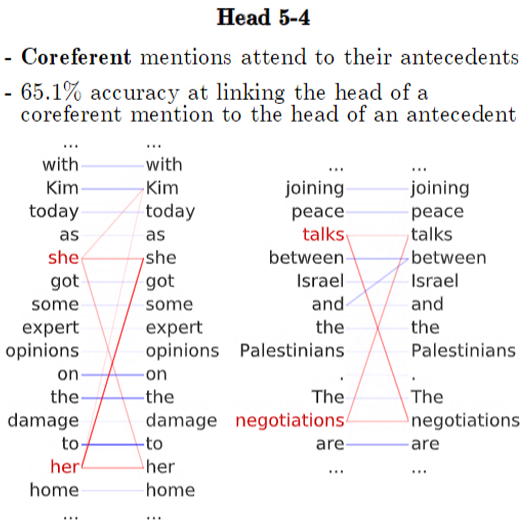
\includegraphics[width=\textwidth]{imgs/bert_headsCoref.png}
  \captionof{figure}{\footnotesize BERT attention heads capture syntax. In heads 5-4, BERT does some \nameref{nlptask:coreferenceresolutionCR} with high accuracy at linking the head of a coreferent mention to the head of an antecedent. From \emph{What Does BERT Look At? An Analysis of BERT's Attention}, by Clark et al., 2019. \url{https://arxiv.org/abs/1906.04341}. Copyright 2019 by Clark et al.}
  \label{fig:bertCoref}
\end{minipage}
\end{figure}


Attention heads 8-10 in \cref{fig:bertHeadDirectObject} learn how direct objects attend to their verbs, and achieves high accuracy at the direct object relation task. The fact that BERT learns this via self-supervision coupled with the heads' propensity for learning syntax may explain BERT's success. Attention heads 5-4 in \cref{fig:bertCoref} perform \nameref{nlptask:coreferenceresolutionCR}. This task is more challenging than syntax tasks since \hyperref[nlptask:coreferenceresolutionCR]{coreference} links span longer than syntax dependencies, and even state-of-the-art models struggle at this task.




\subsubsection{BERT's Limitation In Segment-Level Representation}

Instead of using separator tokens to gather segment-level information, BERT actually views separator tokens \texttt{[SEP]} as ``no-op" or stub operations for attention heads when the head is not needed for a current task. 

\begin{figure}[h]
\vspace{-5pt}
\centering
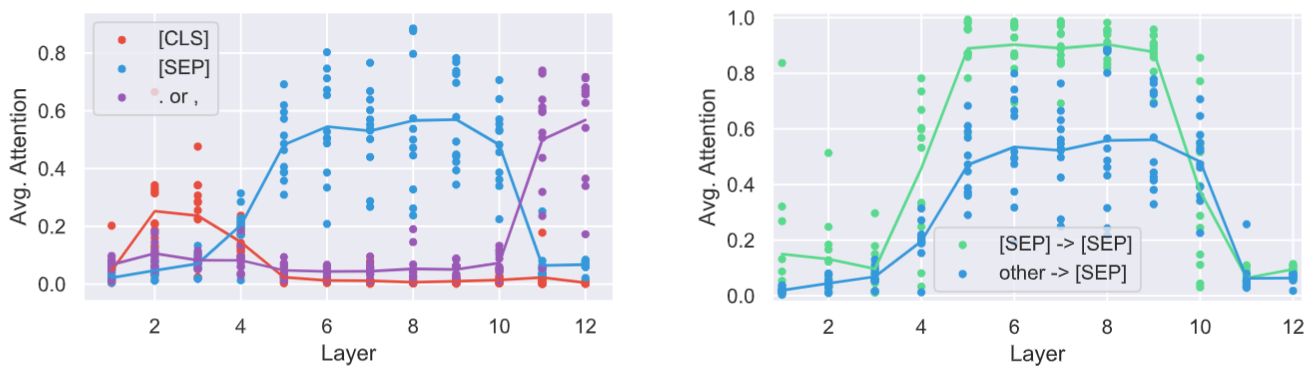
\includegraphics[width=0.95\textwidth]{imgs/bert_attentionheads_SEP.png}
\vspace{-5pt}
\caption{\footnotesize BERT's attention heads in layers 6-10 spend more than half the average attention to separator tokens; deep heads attend to punctuation, while middle heads attend to \texttt{[SEP]}, and early heads attend to \texttt{[CLS]}. From \emph{What Does BERT Look At? An Analysis of BERT's Attention}, by Clark et al., 2019. \url{https://arxiv.org/abs/1906.04341}. Copyright 2019 by Clark et al.}
\vspace{-5pt}
\label{fig:bertSEPAttention}
\end{figure}

Authors hypothesized as to why so many of BERT's attention heads focus on separator tokens, a feature visible in \cref{fig:bertSEPAttention}. But there are several investigations that prove this may not be the case: 
\begin{enumerate}
    \item If BERT were indeed trying to gather segment-level information, then attention heads processing \texttt{[SEP]} should attend broadly over the entire segment to create the segment representations. But \cref{fig:bertHeadDirectObject} shows that in heads 8-10 direct objects attend to their verbs, while all other words attend to the \texttt{[SEP]} token. 
    
    \item Gradient measures were used to study how much the attention to a token would change BERT's outputs. While attention to \texttt{[SEP]} increases from layer 5 onwards (visible in \cref{fig:bertSEPAttention}), the gradients for attention to \texttt{[SEP]} decrease substantially (visible in \cref{fig:bertGradient}). This means attending to \texttt{[SEP]} does not significantly change BERT's outputs. 
\end{enumerate}


\begin{figure}[h]
\vspace{-5pt}
\centering
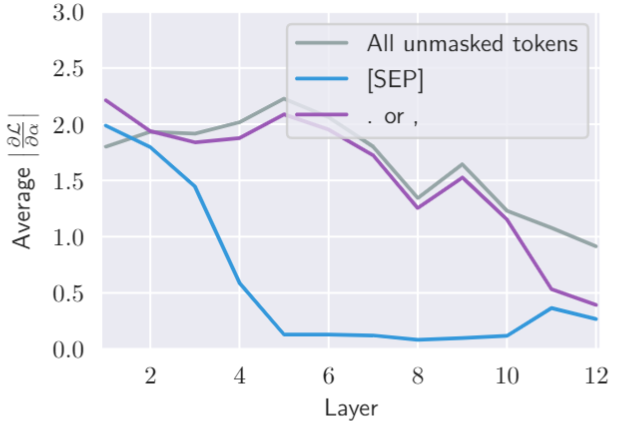
\includegraphics[width=0.45\textwidth]{imgs/bert_attentionheads_gradient.png}
\vspace{-5pt}
\caption{\footnotesize Gradient-based estimates for attention to separator and punctuation tokens. Authors ``compute the magnitude of the gradient of the loss from the \nameref{sec:maskedlanguagemodelMLM} task with respect to each attention weight." From \emph{What Does BERT Look At? An Analysis of BERT's Attention}, by Clark et al., 2019. \url{https://arxiv.org/abs/1906.04341}. Copyright 2019 by Clark et al.}
\vspace{-5pt}
\label{fig:bertGradient}
\end{figure}



The above two investigations suggest BERT's attention heads only attend to \texttt{[SEP]} when they have no other job, not to gather segment-level information. However, \nameref{sec:TransformerXL} by design improves over BERT in this regard. 









\subsubsection{BERT's Contribution To Polysemy} % PAPER: DOEs bert make any sense

Using a kNN classification, Wiedemann et al. (2019) compared the \hyperref[sec:SolutionWithContextEmbs]{contextual embeddings (CWE)s} of \nameref{sec:ELMo} and BERT on the \nameref{nlptask:wordsensedisambiguatioNWSD} task and found that BERT places \hyperref[sec:Polysemy]{polysemic} words into distinct regions according to their senses, while \nameref{sec:ELMo} cannot. Specifically, in \nameref{sec:ELMo} embeddings, major word senses are less strongly separated than in the BERT embedding space, where some senses are sharply clustered. 

In \cref{tbl:bertPolysemy} Wiedemann et al. (2019) also made inferences about the semantic features of BERT's embeddings by studying how BERT matched word senses from the test set to a given \hyperref[sec:Polysemy]{polysemic} word from a training set.



\begin{table}[ht!]
  \centering
  \caption{\footnotesize Example predictions by BERT based on nearest neighbor sentences. The \hyperref[sec:Polysemy]{polysemic} word is \textbf{bolded}, and has a WordNet description tag describing its correct sense to be predicted. {\color{ForestGreen} True positives by BERT are green} while {\color{Red} false positives made by BERT are red}. From \emph{(adapted) Table 4 in Does BERT Make Any Sense? Interpretable Word Sense Disambiguation with Contextualized Embeddings}, by Wiedemann et al., 2019. \url{https://arxiv.org/pdf/1909.10430.pdf}. Copyright 2019 by Wiedemann et al.}
  \begin{tabular}{ c }
    
    \begin{minipage}{.9\textwidth}
      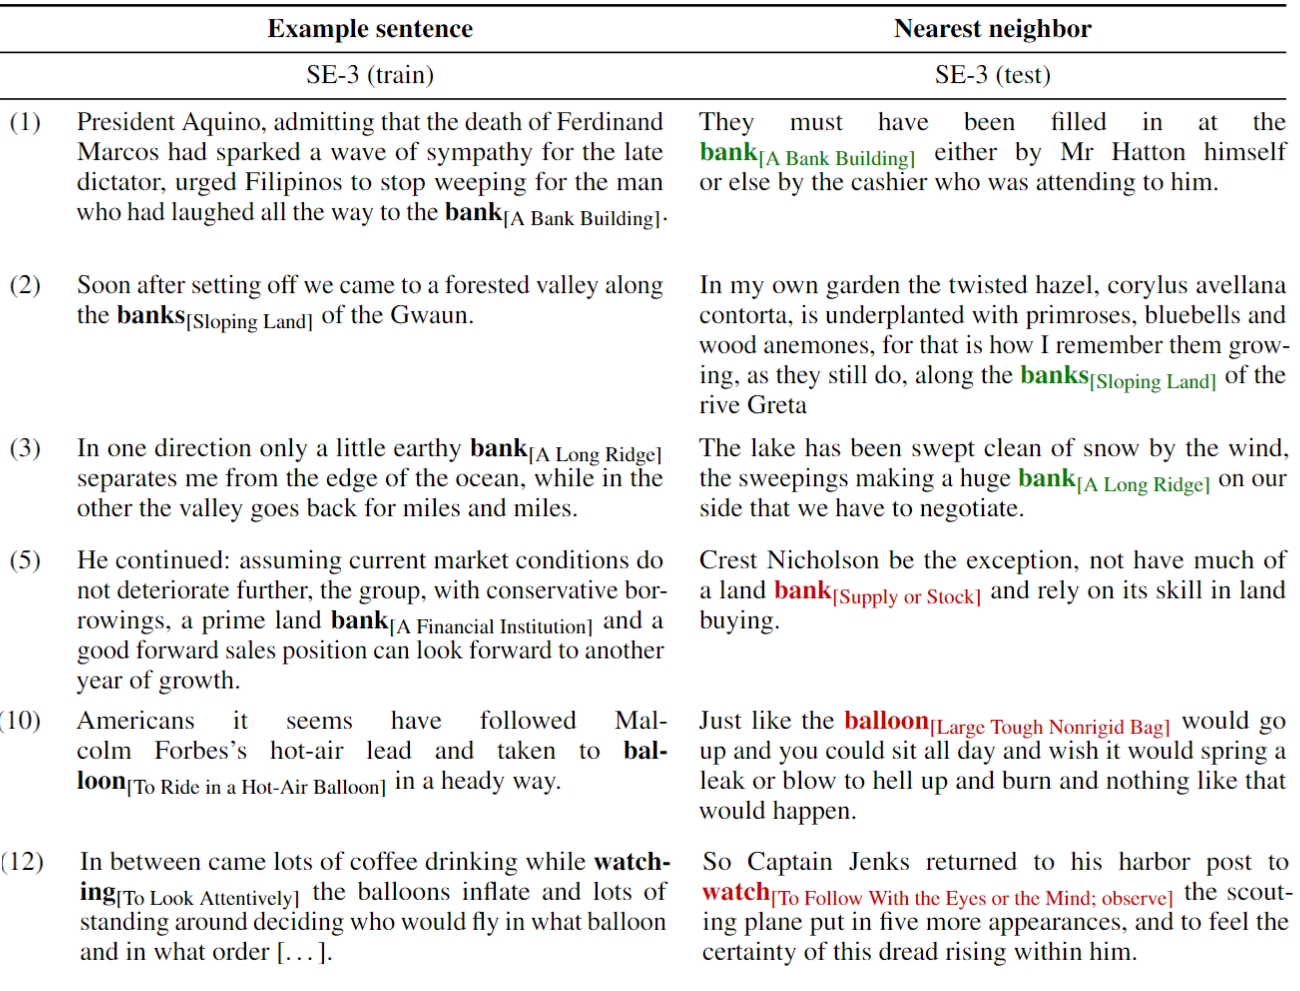
\includegraphics[width=\linewidth]{imgs/table_bertPolysemyTests.png}
    \end{minipage}
    
  \end{tabular}
  \label{tbl:bertPolysemy}
\end{table}



BERT did well when the data had \emph{vocabulary overlap} in context, such as in example (2) ``along the \emph{bank} of the river" (the input text) and `along the \emph{bank} of the river Greta" (nearest neighbor found by BERT). BERT also predicted correctly when text had \emph{semantic overlap}, such as in example (3)'s input ``little earthy bank" and nearest neighbor ``huge bank [of snow]". 

However, \emph{vocabulary and semantic overlap in conjunction} led BERT to make false predictions. Example (5) in \cref{tbl:bertPolysemy} shows BERT predicted ``land bank" as in a \emph{supply or stock} while the correct sense of ``land bank" was \emph{financial institution}. In example (10), the correct word sense of ``balloon" is a verb while BERT predicted a noun sense, so it did not even get the word class correct. Even harder for BERT was to distinguish verb senses correctly; example (12) shows the correct sense label of the \hyperref[sec:Polysemy]{polysemic} word ``watch" was \emph{to look attentively} while BERT's predicted sense was \emph{to follow with the eyes or the mind; observe}. 

Despite BERT's limitations, the authors conclude still that BERT captures \hyperref[sec:Polysemy]{polysemy} more successfully than \nameref{sec:ELMo}, inspiring future work in using \nameref{nlptask:wordsensedisambiguatioNWSD} to compare BERT to models like \nameref{sec:XLNet}. 